\newpage
\subsection{Relaxometry} \label{sec:relax}

The time evolution of magnetization towards equilibrium is characterized by relaxation time constants $T_1$ and $T_2$ for longitudinal and traverse components, respectively. In biological tissues, dipole-dipole interactions serve as the dominant mechanism responsible for relaxation. Field strength and material composition modulate dipole-dipole interactions, hence a wide range of $T_1$ and $T_2$ values can be found for the same nuclear target, e.g. ${}^1 H$.

In this module you will explore several methods for measuring the $T_1$ and $T_2$ of a few basic tissue-mimicking materials. Table \ref{table:relax} lists these materials with empirical measurements of $T_1$ and $T_2$ \textbf{at 1.5 T} from recent literature\footnote{Antoniou, Anastasia, et al. ``MR relaxation times of agar‐based tissue‐mimicking phantoms.'' Journal of Applied Clinical Medical Physics 23.5 (2022): e13533.}.

\begin{table}[!h]
\begin{center}
\begin{tabular}{ |c|c|c| } 
\hline
\textbf{Material} & \textbf{$T_1$ (ms)} & \textbf{$T_2$ (ms)} \\ \hline
Oil & 193 & 55 \\ \hline
Agar & 1670 & 46 \\ \hline
\end{tabular}
\end{center}
\caption{\label{table:relax} Mean $T_1$ and $T_2$ of basic tissue-mimicking materials for proton (${}^1 H$) imaging at 1.5T.}
\end{table}

Note the field strength at which the measurements in Table \ref{table:relax} were collected. In most biological tissues, $T_1$ increases approximately as $B_0^{1/3}$ and $T_2$ is approximately constant over the range of field strength relevant to clinical MRI. \textbf{These are primitive rules of thumb}, but can nevertheless serve as a helpful starting point for designing relaxometry experiments at a novel field strength.

\vspace{5mm}

\color{red} Use the $B_0^{1/3}$ power law and Table \ref{table:relax} to estimate $T_1$ of oil and agar at the field strength of the tabletop system (0.26T).
\color{black}
% soln:
% T1 * (0.26/1.5)^(1/3)
% oil 108ms; agar 931ms; water 1185ms

\vspace{5mm}

\begin{wrapfigure}{r}{0.5\textwidth}
    \vspace{-5mm}
    \centering
    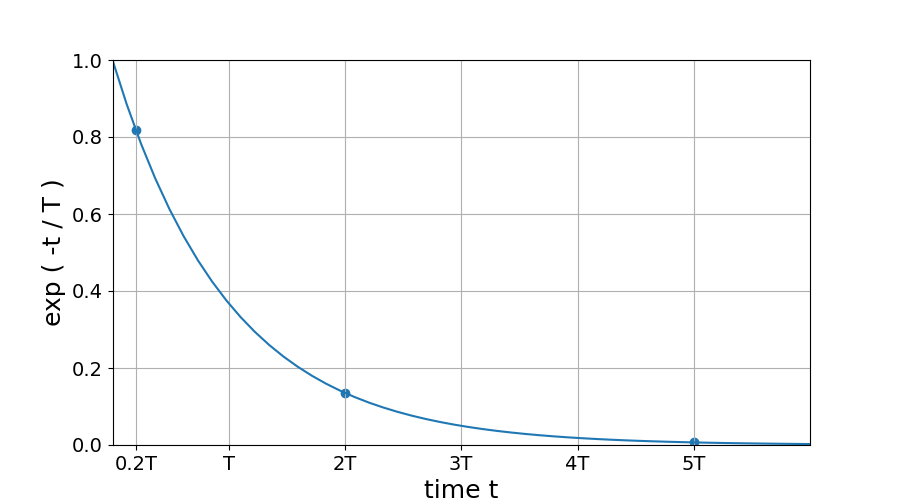
\includegraphics[width=0.5\textwidth]{exp-decay}
    \captionsetup{width=0.4\textwidth}
    \caption{\label{fig:decay} Exponential decay with a generic time constant $T$. This plot can be a helpful reference for designing relaxometry experiments.}
\end{wrapfigure}

In order to measure $T_1$ or $T_2$ you will tune the timing parameters of a spin echo sequence to elicit sensitivity to just one of these time constants at a time. For the sake of both accuracy and efficiency, it will be important to \textbf{design your sampling range to cover the most significant portion of the decay/recovery curve} for the time constant you are measuring. To this end you may find Figure \ref{fig:decay} to be a helpful reference for choosing parameters in proportion to the (expected) time constant value. For example, we can see that the majority of decay/recovery happens during the time window between 20\% and 200\% of the time constant T. By time 5T, decay is practically complete.

\newpage
\subsubsection{Measuring $T_2$} \label{sec:T2}

\emph{Note: B0 homogeneity is very important for $T_2$ measurement accuracy. Check that B0 inhomogeneity is below 50 ppm before continuing. You can check this value by acquiring a spectroscopy spin echo and inspecting the Plotvalues window.}

\vspace{5mm}
Consider the following saturation-recovery spin echo sequence.
\newline \newline
$90^{\circ}$ --- TE/2 --- $180^{\circ}$ --- TE/2 --- DAQ
\newline \newline
We will use this sequence to measure $T_2$ by iterating over a range of echo times (TE) and fitting a mono-exponential to the resulting signal decay curve $s(\text{TE})$. The Relax 2.0 program will actually do this for you by fitting a line to the log of the decay curve.
\vspace{5mm}

\color{red}
Derive an expression for $T_2$ in terms of the slope of the linearized decay, $\log{s}$. Assume complete recovery over each iteration ($\text{TR} \gg T_1$).
\color{black}
\vspace{5mm}
% soln: $T_2 = -1 / slope$

We will now collect data to plot the decay curve and measure $T_2$ for a sample.

\begin{enumerate}
    \item   Install the oil phantom. \emph{Remember to re-calibrate the center frequency as needed}.
    \item   In the main menu, click \textbf{T2 measurement} and select the \textbf{Spin Echo} sequence.
    \item  Open \textbf{Parameters}. Under \emph{General}, set Sampling Time to 6 ms and pick a suitable TR for $T_1$ insensitivity. Under \emph{T2 Measurement}, choose a suitable range of 10 TE values for fitting a $T_2$ decay.
    \item   Click \textbf{Acquire} and wait for the program to run its course.
    \item   Click \textbf{Data Process} and observe the resulting plot.
    \item   Tune your timing parameters as needed to achieve a good fit ($|r| \geq 0.97$). Hint: Figure \ref{fig:decay} can help you pick suitable values for TE and TR.

    \color{red} Report your chosen timing parameters and explain your reasoning.
    \color{black}
    % soln: avoid T_1 contrast with TR >> T_1; TE range around T_2$

    \color{red} 
    Include a screenshot of the resulting plot with $T_2$ and $r$ clearly visible. 
    \color{black}

    \color{red} 
    Use the formula you derived for the slope to validate the $T_2$ value computed by Relax 2.0. Comment on the agreement with Table \ref{table:relax}.
    \color{black} 
    
    % works well with TE range around 10-200% of T2
    \item   Repeat these steps for each material in Table \ref{table:relax}.
\end{enumerate}

\color{red}
You may have noticed that TE values much larger than $T_2$ tend to produce outliers in the linear fit. Explain this effect.
\color{black}
% soln: as transverse signal decays to 0, thermal noise becomes dominant and we lose the mono-exponential shape

\newpage
\subsubsection{Measuring $T_1$} \label{sec:T1}

Consider the following inversion-recovery spin echo sequence. We will use this sequence to measure $T_1$ by iterating over a range of inversion times (TI). \newline
\newline
$180^{\circ}$ --- TI --- $90^{\circ}$ --- TE/2 --- $180^{\circ}$ --- TE/2 --- DAQ
\newline

\color{red}
Sketch the $M_z$ magnetization for one iteration of this sequence, assuming $\text{TR} \gg T_1$. Use your sketch to derive an expression for the $M_z$ null point in terms of $T_1$. Hint: the $M_z$ null point is the time at which $M_z$ crosses through zero after the initial $180^{\circ}$ pulse. 
\color{black}
% soln: TI_null = T_1 log(2) (eqn 7.51 in Nishimura textbook)

We will now collect data to locate the $M_z$ null point for a sample and measure $T_1$:
\begin{enumerate}
    \item   Install the oil phantom. \emph{Remember to re-calibrate the center frequency as needed}.
    \item   In the main menu, click \textbf{T1 measurement} and select \textbf{Inversion Recovery (SE)}.
    \item   Open \textbf{Parameters}. Under \emph{General}, set Sampling Time to 6 ms, pick a suitable TE for $T_2$ insensitivity, and pick a suitably long TR for full recovery. Under \emph{T1 Measurement}, choose a suitable range of 10 TI values to locate the $M_z$ null point.
    \newline
    \color{red} Report your chosen timing parameters and explain your reasoning.
    \color{black}
    % soln: TR >> T_1; TE << T_2; TI range should include expected null-point at T_1 log(2)$
    \item   Click \textbf{Acquire} and wait for the program to run its course.
    \item   Click \textbf{Data Process} and observe the resulting plots. Ignore the fit lines and reported $T_1$ value for now - these will likely be way off.
    \newline
    \color{red}
    Record the approximate TI value achieving minimum signal amplitude among the 10 points. Take this TI value as the $M_z$ null point to estimate $T_1$ using the formula you derived above.
    \color{black}
    % soln: T_1 = TI_null / log(2)

    \item Finally, we will measure $T_1$ again but this time by fitting a mono-exponential to the recovery curve. The \textbf{Data Process} routine actually does this for you by fitting a line to the log of the recovery curve $s(\text{TI})$. To be precise, the Relax 2.0 software actually fits a line to $\log{(\text{max}(s)-|s|)}$. This is a rather precarious implementation choice, but it should work well enough for our purpose so long as the following conditions are met:
    \begin{itemize}
        \item TI range begins \emph{after} the $M_z$ null point
        \item $\text{max}(s)$ is close to the equilibrium magnetization, i.e. $\text{max}(\text{TI}) \gg T_1$
    \end{itemize}
    
    With these conditions in mind, tune your timing parameters to achieve a good fit ($|r| \geq 0.97$) with 10 values for TI. One more hint: choose TR such that $\text{TR} - \text{max}(\text{TI}) \gg T_1$ to ensure adequate signal recovery in all cases.
        
\color{red}
Report your chosen timing parameters and explain your reasoning.
\color{black}
% works well with TI range 100-500% of T1

\color{red}
Attach screenshots of the two resulting plots with $T_1$ and r-value clearly visible.
\color{black}
% soln: In addition to the guidance provided in the hints (TI_max >> T1, TR - TI_max >> T1), want TE << T2 and TI spanning the significant portion of the recovery curve.

    \item   Repeat these steps for each material in Table \ref{table:relax}.

\end{enumerate}

\color{red}
Now you have tried three different methods for estimating $T_1$ in a variety of materials. Comment on the degree of agreement and relative accuracy across these methods.
\color{black}





